\chapter{Simpson's Paradox}
This chapter 
is based on Chapter 6 of 
``The Book of Why", Ref.\cite{book-why}.
See also
Ref.\cite{wiki-simpson}
and references therein.


Simpson's paradox is a recurring 
nightmare for all statisticians 
overseeing a clinical trial for 
a medicine. It is possible that
 if they leave out a certain 
"confounding" variable from a study, 
the study's conclusion on whether
 a medicine is effective or not, might be,
 without measuring that confounding variable, 
the opposite of what it would have 
been had that variable been measured.

Simpson's Paradox is greatly clarified
 by Judea Pearl's theory of causality.
 At the end of this chapter, 
we explain how.

Here is a simple example of 
Simpson's Paradox.

An equal 
number of  patients of male and 
female genders
 are given a heart medicine or a placebo 
in a double blind study.
 Some subsequently have a heart 
attack. Let

$ \ul{a}=$ heart attack? No=0, Yes=1

$ \ul{t}=$ took medicine? No=0, Yes=1

$ \ul{g}=$ gender? Female=0, Male=1



\begin{figure}[h!]
\centering
$$\xymatrix{
&\rvg\ar[dl]&\\
\rva&&\ul{\rvt}\ar[ul]\ar[ll]
}$$
\caption{bnet for a simple example of 
Simpson's paradox.
Here node $\rvg$ is 
a chain junction and a mediator.}
\label{fig-simpson-chain}
\end{figure}

\begin{figure}[h!]
\centering
$$\xymatrix{
&\rvg\ar[dl]\ar[dr]&\\
\rva&&\ul{\rvt}\ar[ll]
}$$
\caption{bnet that is probabilistically
but not physically
equivalent to bnet
Fig.\ref{fig-simpson-chain}.
Here node $\rvg$ is 
a fork junction and a confounder.}
\label{fig-simpson-fork}
\end{figure}




This situation can be modeled by 
either
bnet Fig.\ref{fig-simpson-chain}.
or bnet
 Fig.\ref{fig-simpson-fork}.
The two bnets are 
probabilistically
equivalent 
(i.e., they
both represent the same
probability distribution $P(a, t, g)$)
because

\beq
P(g|t)P(t)=P(g,t)=P(t|g)P(g)
\;.
\eeq

For the bnet
Fig.\ref{fig-simpson-chain}, 
one has

\beq
P(a,g,t)=P(a|g,t)P(g|t)P(t)
\;.
\eeq
Therefore,

\beq
P(a=1|t)=
\sum_g P(a=1|t, g)P(g|t)=E_{\ul{g}|t}
P(a=1|t, \ul{g})
\;,
\eeq
where $ E_{\ul{g}|t}$ is 
a conditional expected value
 (a kind of weighted average).

Suppose $ q_0, q_1$ are 
non-negative real numbers. 
For the vector $ \vec{q}=(q_0, q_1)$:

Define a negative outcome 
(or failure or $ q_t$ 
increasing with $ t$) 
if $ q_0 \leq q_1$.

Define a positive outcome 
(or success or $ q_t$ 
decreasing with $ t$)
 if $ q_0 \geq q_1$.

Let

\beq
\vec{q}^{\;g}=
[P(\rva=1|t,g)]_{t=0,1}
\;
\eeq
for $g=0,1$, and

\beq
\vec{q}^{\;*}=[P(\rva=1|t)]_{t=0,1}
\;.
\eeq

\begin{figure}[h!]
\centering
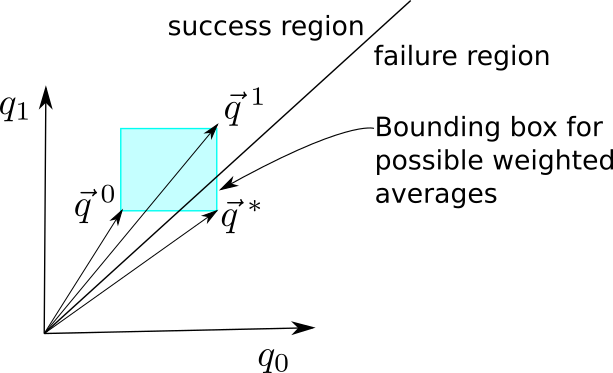
\includegraphics[width=3.5in]
{simpson/q-vecs.png}
\caption{$\vec{q}^{\;0}$,
$\vec{q}^{\;1}$ vectors
and bounding box for vector $\vec{q}^{\;*}$.  } 
\label{fig-simpson-q-vecs}
\end{figure}

It is possible (see Fig.\ref{fig-simpson-q-vecs} 
for a graphical explanation of how)
 to find perverse cases in which
 $ P(a=1|t, g=0)$ and $ P(a=1|t, g=1)$
 increase with $ t$ but $ P(a=1|t)$ 
decreases with $ t$. So it is possible 
to conclude that the medicine is a failure
 for each of the two $ g$ populations 
considered separately, yet the medicine 
is a success when both populations are 
``amalgamated". The lesson is that a
 ``trend reversal" is possible 
upon amalgamation. Trends
are not necessarily preserved 
when we do a weighted average of
 type $ E_{\ul{g}|t}$. 
$ E_{\ul{g}|t}$ is an expected value
 on the random variable $ \ul{g}$
 conditioned on the root 
random variable $ \ul{t}$.


So far, we have proven that probabilistically, 
the drug can be a failure for the populations
 of both sexes considered separately, 
but a success for the aggregate population.

\section{Pearl Causality}

Pearl Causality would add 
the following two 
important insights 
to this problem:
\begin{enumerate}
\item bnets Fig.\ref{fig-simpson-chain} 
and Fig.\ref{fig-simpson-fork}, 
although they are
probabilistically equivalent, 
do not represent the same physical
 situation. In fact, only
 Fig.\ref{fig-simpson-fork} 
occurs in this case.
\item To decide whether the
 medicine is effective, we 
must apply a $do()$ operator to
 the $\rvt$ variable in
 Fig.\ref{fig-simpson-fork}. 
The effect of that $do()$ operator
 is to erase the arrow going 
from $ \rvg$ to $ \rvt$. This in turn means
 that the average $ E_{\ul{g}|t}$
 in our equation for $ P(a=1|t)$
 becomes a simpler average $ E_{\ul{g}}$
 which is independent of $ \rvt$. 
But for such an average,
 the
 bounding box in Fig.\ref{fig-simpson-q-vecs}
 degenerates to its diagonal 
line that connects the tips
 of the two vectors $ \vec{q}^{\;0}$
 and $ \vec{q}^{\;1}$. The vector 
$ \vec{q}^{\;*}$ must now fall on 
that diagonal line and must therefore
 also fall in the success region.
\end{enumerate}
In conclusion, as Judea Pearl would say,
 if we ask the right question to Nature,
 i.e., what is
 $ P[a=1 | do(\ul{t}=t)]$ for $ t=0,1$,
 we get as an answer that the 
aggregate population preserves 
rather than reverses the
 unanimous trend of the 
two gendered populations.
\newpage
\section{Numerical Example}

\begin{table}[h!]
\centering
\begin{tabular}{|l|l|l|}
\hline
\rowcolor[HTML]{ECF4FF} 
$(a,t,g)$ & \begin{tabular}[c]{@{}l@{}}number of patients\\ segregated by gender\end{tabular} & \begin{tabular}[c]{@{}l@{}}number of patients\\ of either gender\end{tabular} \\ \hline
0,0,0 & 19 & 47 \\ \cline{1-2}
0,0,1 & 28 &  \\ \hline
0,1,0 & 37 & 49 \\ \cline{1-2}
0,1,1 & 12 &  \\ \hline
1,0,0 & 1 & 13 \\ \cline{1-2}
1,0,1 & 12 &  \\ \hline
1,1,0 & 3 & 11 \\ \cline{1-2}
1,1,1 & 8 &  \\ \hline
\end{tabular}
\caption{Data for numerical example 
 of Simpson's Paradox. This 
fictitious data was taken directly
 from Table 6.4, page 210
of ``The Book of Why", 
Ref.\cite{book-why}.}
\label{tab-simpson-heat-attack}
\end{table}

\beq
P(a|t,g)=
\begin{array}{c|cccc}
&\scriptstyle 0,0 & \scriptstyle 0,1 &
\scriptstyle  1,0 &\scriptstyle 1,1\\\hline
\scriptstyle  0& 19/20 & 28/40 & 37/40 & 12/20\\
\scriptstyle 1& 1/20 & 12/40 & 3/40 & 8/20
\end{array}
\eeq

\beq
P(a|t)=
\begin{array}{c|cc}
&\scriptstyle 0 & \scriptstyle 1\\\hline
\scriptstyle 0& 47/60& 49/60\\
\scriptstyle  1& 13/60 & 11/60
\end{array}
\eeq

\beq
\begin{array}{lll}
\frac{
P(a=1,t=1, g=0)
}{
\sum_aP(a, t=1, g=0)
}=
P(a=1|t=1, g=0) &=& \frac{3}{40}
\\
\frac{
P(a=1,t=0, g=0)
}{
\sum_aP(a, t=0, g=0)
}=
P(a=1|t=0, g=0) &=& \frac{1}{20}=\frac{2}{40}
\end{array}
\label{eq-g-eq-0}
\eeq

\beq
\begin{array}{lll}
\frac{
P(a=1,t=1, g=1)
}{
\sum_aP(a, t=1, g=1)
}=
P(a=1|t=1, g=1) &=& \frac{8}{20}=\frac{16}{40}
\\
\frac{
P(a=1,t=0, g=1)
}{
\sum_aP(a, t=0, g=1)
}=
P(a=1|t=0, g=1) &=& \frac{12}{40}
\end{array}
\label{eq-g-eq-1}
\eeq

\beq
\begin{array}{lll}
\frac{
\sum_g P(a=1,t=1, g)
}{
\sum_g\sum_aP(a, t=1, g)
}=
P(a=1|t=1) &=& \frac{11}{60}
\\
\frac{
\sum_g P(a=1,t=0, g)
}{
\sum_g\sum_aP(a, t=0, g)
}=
P(a=1|t=0) &=& \frac{13}{60}
\end{array}
\label{eq-g-eq-all}
\eeq

Note
that the right hand
side
of 
Eq.(\ref{eq-g-eq-0})
is higher
for $t=1$
than for $t=0$.
Same trend 
occurs
in Eqs.\ref{eq-g-eq-1}
but
is reversed in Eqs.\ref{eq-g-eq-all}.